\section*{Exercice 168 -- Train épicycloïdal}

\setcounter{exo}{0}

Soit le train épicycloïdal suivant. 

\begin{center}
 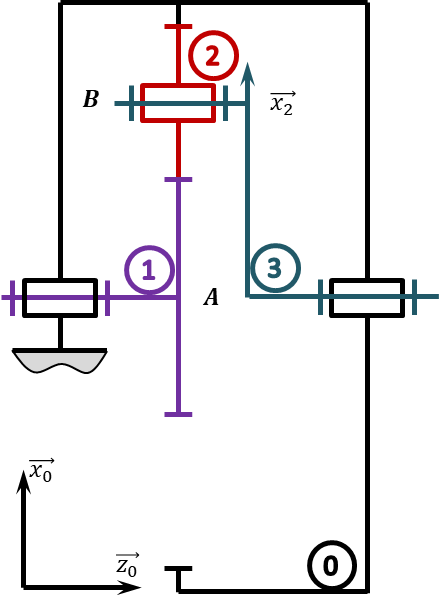
\includegraphics[width=.6\linewidth]{047_01}
\end{center}



\subparagraph{}
\textit{Déterminer le rapport de réduction $\dfrac{\omega_{30}}{\omega_{10}}$.}
 \ifprof
 \begin{corrige}
 
 En bloquant le porte satellite, on a : $\dfrac{\omega_{03}}{\omega_{13}}=-\dfrac{Z_1}{Z_0}$. On a donc, 
$\dfrac{\omega_{03}}{\omega_{10}+\omega_{03}}=-\dfrac{Z_1}{Z_0}$

$\Leftrightarrow \dfrac{\omega_{30}}{\omega_{30}-\omega_{10}}=-\dfrac{Z_1}{Z_0}$
$\Leftrightarrow \omega_{30}=-\dfrac{Z_1}{Z_0} \omega_{30}+\dfrac{Z_1}{Z_0}\omega_{10} $
$\Leftrightarrow \omega_{30}\left( 1+\dfrac{Z_1}{Z_0} \right)=\dfrac{Z_1}{Z_0}\omega_{10} $
$\Leftrightarrow \omega_{30}=\dfrac{Z_1}{Z_0+Z_1}\omega_{10} $
 \end{corrige}
 \else
 \fi

